\section{Ranking under uncertainty}\label{sec:17.6}

Paratellurite, TeO$_2$, has the softest lattice of the crystals we rank: its effective sound speed $c_{\mathrm{NR1}}$, the inverse of its heavy-mediator figure of merit (\cref{sec:17.5}), is \SI{3.75}{km/s}, against \SI{4.58}{km/s} for CaWO$_4$ and \SI{8.96}{km/s} for silicon. Its single-phonon rate per unit mass should then be 2.39 times silicon's, and 1.22 times that of CaWO$_4$. The speeds of CaWO$_4$ and TeO$_2$ have different origins, however. The speed of CaWO$_4$ follows from an ultrasonic measurement of its elastic tensor; the speed of TeO$_2$ follows from a tensor computed with a density functional, whose errors are of order \SI{10}{\percent} and are not stated with the number. Whether TeO$_2$ beats CaWO$_4$ depends on those errors.

\subsection{Provenance widths}\label{sec:17.6-widths}

Every input of a figure of merit is one of three kinds. A \emph{measured} input comes from an experiment on the crystal: the low-temperature gap of silicon, \SI{1.17}{eV} (\cref{tab:3-materials}), or the elastic constants of germanium, 131, 49 and \SI{68}{GPa} (\cref{sec:11.1}). A \emph{computed} input comes from a first-principles calculation, such as the elastic tensors of a materials database or the Born charges of a density-functional perturbation calculation. An \emph{estimated} input is a parametric guess or a prior, such as the shift of a gap from room temperature to the millikelvin temperatures of a detector. We give each input a lognormal distribution, $\ln x_j$ Gaussian about $\ln x_{j0}$ with width $\sigma^{\mathrm{prov}}_j$, or a stated uniform prior. The provenance width $\sigma^{\mathrm{prov}}_j$ is a convention, set by the kind of input rather than worked out number by number; \cref{tab:17-widths} lists the values we use.

\begin{table}[tbp]
  \caption{Provenance widths: the Gaussian width $\sigma^{\mathrm{prov}}_j$ of $\ln x_j$, or the prior, assigned to each kind of input of a figure of merit. The values are conventions. The widths for computed sound speeds and for room-temperature gaps are tested against the book's crystals in \cref{sec:17.6-widths}; the prior on $X_{\mathrm{pole}}$ is a device (\cref{sec:17.6-correlation}).}
  \label{tab:17-widths}
  \centering\footnotesize\setlength{\tabcolsep}{4pt}
  \begin{tabular}{@{}>{\raggedright\arraybackslash}p{0.30\linewidth}>{\raggedright\arraybackslash}p{0.36\linewidth}>{\raggedright\arraybackslash}p{0.26\linewidth}@{}}
    \toprule
    Kind of input & Example & Width \\
    \midrule
    Measured, spread stated & sapphire $\mathcal{I}_{\mathrm{pol}}$ through $\varepsilon_\infty = 3.1$--3.3; GaAs $\mathcal{I}_{\mathrm{pol}}$, half the spread of its dielectric and splitting routes & 0.03; 0.04 \\
    Measured, no error stated & gap at low temperature; speed from a measured tensor; frequency of a measured phonon & 0.01; 0.02; 0.005 \\
    Measured at room temperature, used at low temperature & gap of a crystal without low-temperature data & room-temperature value plus a shift uniform on 0.03--\SI{0.10}{eV} \\
    Computed, materials database & sound speed from a computed elastic tensor; density of a computed cell & 0.086; 0.030 \\
    Computed, density-functional perturbation theory & Born charge $Z^*$, $\varepsilon_\infty$; optical-phonon energy & 0.07; 0.05 \\
    Estimated & interband enhancement $X_{\mathrm{pole}}$ of the Migdal pole factor & log-uniform on [1, 3] \\
    \bottomrule
  \end{tabular}
\end{table}

Two widths decide most of the rankings, and the book's own crystals test both. For computed sound speeds we take the elastic tensors of the JARVIS (Joint Automated Repository for Various Integrated Simulations) database, obtained with one exchange--correlation functional, OptB88vdW, for every crystal~\cite{choudhary2018elastic}. Silicon, germanium and diamond have measured tensors (\cref{sec:11.1}), so the database can be compared with experiment on the same quantity. Solving the Christoffel problem for the database and the measured tensors gives database values of $c_{\mathrm{NR1}}$ below the measured ones by \SI{2.9}{\percent} for silicon, \SI{10.2}{\percent} for germanium and \SI{1.0}{\percent} for diamond. The root mean square of the logarithmic differences is 0.065, inside the width 0.086 we assign. All three differences have the same sign, however, with a mean of $-0.048$: the errors of one method are not independent from crystal to crystal (\cref{sec:17.6-correlation}). For gaps, the shift from room temperature to low temperature is 0.05, 0.08 and \SI{0.10}{eV} for silicon, germanium and GaAs (\cref{tab:3-materials}); a crystal whose gap is known at room temperature alone gets a shift drawn uniformly between 0.03 and \SI{0.10}{eV}. Neither width is a bound: a crystal whose computed tensor errs by \SI{25}{\percent}, or whose gap moves by \SI{0.2}{eV} on cooling, is not excluded by the convention.

The halo enters every edge through the same power of $v_{\mathrm{max}}$, so a common factor on $v_{\mathrm{max}}$ multiplies all edges alike and changes no order in any draw. We keep $v_{\mathrm{max}} = 2.650\times10^{-3}$ fixed.

Our pool of crystals consists of silicon, germanium, GaAs and diamond, and seven insulators that cryogenic experiments use or propose: sapphire, LiF, NaF, CaWO$_4$, TeO$_2$, Li$_2$MoO$_4$ and $\gamma$-LiAlO$_2$. Each probability below is taken over this pool. The gaps of silicon, germanium and GaAs are the low-temperature values 1.17, 0.744 and \SI{1.52}{eV} of \cref{tab:3-materials}, and the gap of diamond, 5.47~eV, is a low-temperature value as well; sapphire (8.8~eV), CaWO$_4$ (5.2~eV), NaF (11.5~eV) and LiF (14.2~eV) enter with room-temperature gaps~\cite[Table~I]{griffin2020multichannel}. The tensors of silicon, germanium and diamond are the measured ones of \cref{sec:11.1}, and CaWO$_4$ enters with the measured tensor of \cref{sec:17.5-phonon}. GaAs, sapphire, TeO$_2$, $\gamma$-LiAlO$_2$, LiF and NaF enter with database tensors and the densities of their computed cells; Li$_2$MoO$_4$ has no tensor in the database and is not ranked in the two channels that need one, the heavy-mediator single-phonon rate and the nuclear edge. The polar inputs of GaAs and sapphire are those of \cref{sec:11.2}: $\mathcal{I}_{\mathrm{pol}}/\rho_T = 0.1415$ for GaAs (the splitting route of \cref{we:11-ipol}) and 9.12 for the ordinary axis of sapphire, both from measured frequencies. For LiF and NaF, \cref{eq:11.2-diatomic} gives 19.0 and $\SI{9.95}{meV.cm^3.g^{-1}}$ with the computed $Z^* = 1.05$ and 0.98, $\varepsilon_\infty = 2.02$ and 1.78, and highest optical energies 77.2 and \SI{49.9}{meV}~\cite[Table~I]{griffin2020multichannel}.

\subsection{Monte Carlo rank statistics}\label{sec:17.6-mc}

With every input a distribution, the figure of merit of each material is sampled by Monte Carlo as in \cref{app:C.14}: we draw $N_{\mathrm{MC}} = 2\times10^4$ sets of inputs, evaluate the figure of merit of every material on each set, and record the order in every draw.

\begin{keyresult}[Ranking under uncertainty]
For each material $A$ of a pool and each draw $k$ of the inputs, let $R_A^{(k)}$ be the rank of $A$ in that draw. Then
\begin{equation}
  P_A(\mathrm{first}) = \frac{1}{N_{\mathrm{MC}}}\sum_{k=1}^{N_{\mathrm{MC}}}\mathbb{1}\bigl[R_A^{(k)} = 1\bigr] , \qquad
  \text{rank interval} = \bigl[R_A^{16}, R_A^{84}\bigr] ,
  \label{eq:17.6-pfirst}
\end{equation}
where $R_A^{16}$ and $R_A^{84}$ are the 16th and 84th percentiles of $R_A^{(k)}$. The tier of $A$ is its height $h(A)$, \cref{eq:C.13-height}, in the interval order \cref{eq:C.13-order} of the 68\% intervals of the figure of merit. All three quantities are conditional on the provenance widths of \cref{tab:17-widths}.
\end{keyresult}

The probabilities $P_A(\mathrm{first})$ sum to one over the pool in every channel, and the sampling error of each is at most $[p(1 - p)/N_{\mathrm{MC}}]^{1/2} \le 0.0035$.

The probability of ranking first measures whether the widths can overturn a lead, not how large the lead is. TeO$_2$ leads the heavy-mediator channel with $P(\mathrm{first}) = 0.968$, and its 68\% interval of $c_{\mathrm{NR1}}(\mathrm{Si})/c_{\mathrm{NR1}}$ is $[2.19, 2.60]$; CaWO$_4$, measured, has the narrow interval $[1.92, 2.00]$ and $P(\mathrm{first}) = 0.010$. With the computed-speed width doubled to 0.172, TeO$_2$ falls to $P(\mathrm{first}) = 0.781$ and GaAs, also computed, rises from 0.022 to 0.135, while CaWO$_4$ gains just from 0.010 to 0.073.

The rank interval says where a material stands when it does not lead. Silicon, in the same channel, has the rank interval 8--8: it is eighth in at least 68\% of the draws, ahead only of sapphire and diamond, whose lattices are stiffer. CaWO$_4$ and GaAs share the interval 2--3. A rank interval that spans several places marks a material whose position the inputs do not fix; the interval says nothing about which neighbor the material trades places with.

\begin{figure}[tbp]
  \centering
  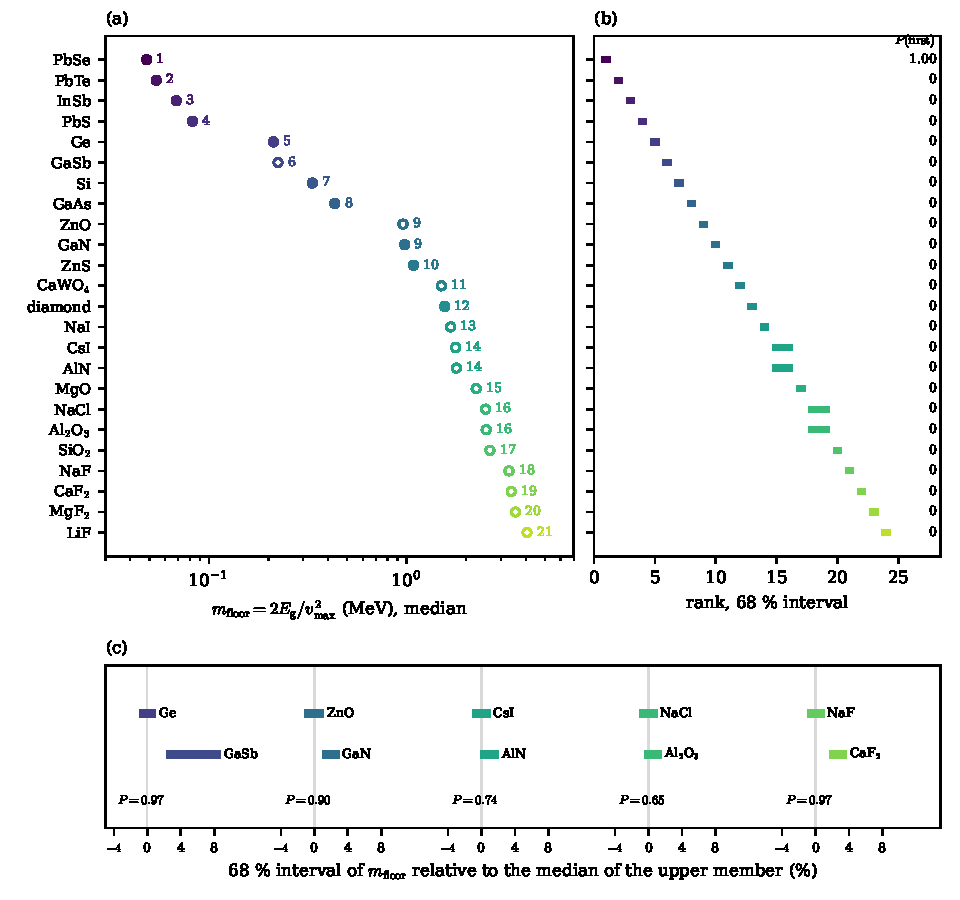
\includegraphics[width=\linewidth]{figures/ch17/fig17_5.pdf}
  \caption{Rank intervals for the electron-recoil floor $2\Eg/v_{\mathrm{max}}^2$, $v_{\mathrm{max}} = 2.650\times10^{-3}$, of the 24 crystals in the target table of Griffin and collaborators~\cite[Table~I]{griffin2020multichannel}, with the low-temperature gaps of \cref{tab:3-materials} for silicon, germanium and GaAs. (a)~Median floor; filled symbols: gap measured at low temperature, open symbols: room-temperature gap plus an upward shift drawn uniformly on 0.03--\SI{0.10}{eV}; gap width 0.01 in the logarithm for all. Numbers and colors: tier (height in the interval order of the 68\% intervals). (b)~Rank, 16th to 84th percentile over $2\times10^4$ draws, and the probability of ranking first. (c)~The 68\% intervals of five close pairs, relative to the median of the member with the lower floor, with the probability $P$ that this member has the lower floor. Pairs in one tier overlap; pairs in different tiers do not, whatever $P$.}
  \label{fig:17-rank-floor}
\end{figure}

\Cref{fig:17-rank-floor} shows the electron-recoil floor $2\Eg/v_{\mathrm{max}}^2$, the lightest mass at which dark matter can cross the gap (\cref{eq:1.3-mmin}), over the 24 crystals of the target table, a wider list than our pool. The lead salts and InSb, whose gaps lie below \SI{0.3}{eV}, hold the four lowest floors, with PbSe at \SI{0.0484}{MeV} and $P(\mathrm{first}) = 1.000$. Germanium is fifth at \SI{0.212}{MeV}, silicon seventh at \SI{0.333}{MeV}. Gaps measured to a percent separate almost every pair, and the 24 crystals fall into 21 tiers. Germanium beats GaSb with probability 0.973, but only because GaSb's gap, \SI{0.720}{eV}, is a room-temperature value and is shifted upward: unshifted, the GaSb floor of \SI{0.205}{MeV} would lie below the germanium floor. With the shift drawn from 0 to \SI{0.15}{eV} instead, the probability falls to 0.837. The order of these two crystals is a statement about the temperature dependence of a gap that has not been measured at the detector's temperature.

Within our pool the electron-recoil floor ranks without ambiguity: germanium, silicon, GaAs, CaWO$_4$, diamond, sapphire, NaF and LiF, each in its own tier and with a rank interval of one place, from \SI{0.212}{MeV} to \SI{4.06}{MeV}. TeO$_2$, Li$_2$MoO$_4$ and $\gamma$-LiAlO$_2$ are not ranked, because no measured gap enters the tables we use.

\subsection{Tiers}\label{sec:17.6-tiers}

A probability of ranking first is a property of one material against the whole pool. To group all materials into classes that the uncertainties can tell apart, we need more: two materials should share a class when their intervals overlap, and be in different classes otherwise. Overlap is not transitive, so no grouping into tied classes can satisfy both conditions in general (\cref{app:C.13}). The interval order resolves the conflict. Material $A$ is resolved above $B$ when the whole 68\% interval of $A$ lies on the better side of the whole interval of $B$, \cref{eq:C.13-order}, and the tier of a material is its height in this order, one plus the length of the longest chain of materials resolved above it, \cref{eq:C.13-height}. Each tier is an antichain, so its members are tied in the exact sense that none is resolved from any other. Every member of tier $k > 1$ is resolved below some member of tier $k - 1$.

A material with a wide interval can therefore rank in a better tier than one with a better median. The nuclear edge $m_{\mathrm{min}}^{\mathrm{ac}}$ at $\omega_{\mathrm{th}} = \SI{1}{meV}$, \cref{eq:11.1-edge} with $c_{\mathrm{LA,max}}$, puts GaAs, with a computed tensor and the interval 10.3--\SI{12.3}{keV}, in tier 6. It puts CaWO$_4$, measured at 10.8--\SI{11.2}{keV}, in tier 7, although the median edge of CaWO$_4$, \SI{11.0}{keV}, is the lower of the two medians. Nothing is resolved between GaAs and germanium, whose measured edge is 10.0--\SI{10.4}{keV}, while germanium is resolved above CaWO$_4$. Tiers add no order that the intervals do not contain, and they discard the information about medians that $P(\mathrm{first})$ keeps; \cref{fig:17-rank-floor}c shows both the tiers and the probabilities. ZnO and GaN share a tier although ZnO has the lower floor with probability 0.90, and NaF and CaF$_2$ are in different tiers, with probability 0.97 that NaF has the lower floor. The tier boundary falls where the intervals stop overlapping, not at a fixed probability.

\subsection{Correlated method errors}\label{sec:17.6-correlation}

The three database speeds that we could check against experiment were all low. If a method errs in the same direction for every crystal, the ratio of two of its results is more accurate than either result, and treating the errors of the two results as independent understates how well the method ranks the two crystals. We model the shared part of the errors with one parameter, the method correlation $r_{\mathrm{mat}}$. Each input of a computed kind draws its Gaussian variable as
\begin{equation}
  z_j = r_{\mathrm{mat}}^{1/2}\,z_{\mathrm{method}} + (1 - r_{\mathrm{mat}})^{1/2}\,z_{j}' ,
  \label{eq:17.6-zmethod}
\end{equation}
with $z_{\mathrm{method}}$ common to every crystal computed with the same method and $z_j'$ the input's own variable, both standard normal. The marginal of every input is unchanged, so are the medians and the 68\% intervals, and so are the tiers built from them, which do not depend on the correlation. Joint statements change. One variable $z_{\mathrm{method}}$ is shared within each of these groups: the database speeds, the densities of computed cells, each quantity of the perturbation calculations, the room-to-low-temperature shift of the gaps and the pole prior $X_{\mathrm{pole}}$. Inputs measured independently never share one. By \cref{eq:C.14-pairwise} the variance of $\ln(x_A/x_B)$ is $\sigma_A^2 + \sigma_B^2 - 2r_{\mathrm{mat}}\sigma_A\sigma_B$, which vanishes at $r_{\mathrm{mat}} = 1$ for two inputs of one method and equal widths.

Correlation sharpens comparisons inside a method. TeO$_2$ beats GaAs, both from database tensors, with probability 0.976 at $r_{\mathrm{mat}} = 0$, 0.997 at 0.5 and 1.000 at 1. Its probability of ranking first rises from 0.968 to 0.985 and 0.987, since its strongest challenger in the draws, GaAs, now moves with it. LiF beats NaF in the polar rate, both through computed Born charges, with probability 0.987 at independent errors and 1.000 at full correlation.

Correlation also resolves ties that the data do not resolve. The Migdal figure of merit is known only between two limits, the plasmon pole and a loss function concentrated at the gap, which differ by $5.7\times10^5$ for silicon (\cref{sec:17.5-migdal}). We rank with the pole form \cref{eq:17.5-pole} times a factor $X_{\mathrm{pole}}$ for the interband weight below the plasma frequency, drawn log-uniformly between 1 and 3. This prior is a device, not a description of the uncertainty. For silicon, the one crystal with a computed spectrum, the plasmon carries \SI{4}{\percent} of the Migdal probability (\cref{sec:12.3}), so the $X_{\mathrm{pole}}$ of silicon is about 25, and $X_{\mathrm{pole}}$ depends on the gap, which differs from crystal to crystal. The medians of the Migdal row are therefore artifacts of the prior, and the order is open, not merely unresolved. At $r_{\mathrm{mat}} = 0$ six crystals share tier 1 and no crystal ranks first with probability above 0.315 (NaF; then silicon 0.290, LiF 0.147). At $r_{\mathrm{mat}} = 1$ the prior cancels from every ratio and NaF ranks first with probability 1.000, although the figure of merit of NaF exceeds that of silicon by \SI{2.4}{\percent}. The resolution at $r_{\mathrm{mat}} = 1$ rests on the assumption of one interband factor for every crystal. We read rankings at $r_{\mathrm{mat}} = 0$ and report the correlated variant beside them: where the independent and the correlated rankings disagree, the ranking rests on an assumption about the method, not on the inputs.

No correlation helps when one material is measured and the other computed. Germanium has a measured tensor and GaAs a database one, and GaAs has the larger figure of merit with probability 0.887. The database speeds of silicon, germanium and diamond are low by \SI{4.9}{\percent} on average; applied to GaAs, this offset lowers the GaAs figure of merit from 1.87 to 1.78 and the probability to 0.744. The same offset on TeO$_2$ lowers the probability that it beats the measured CaWO$_4$ from 0.987 to 0.955. The comparison of a measured with a computed value carries the offset of the method in full, and only a measurement of the crystal with the computed value removes the offset.

\subsection{Rankings of the scattering channels}\label{sec:17.6-rankings}

\Cref{tab:17-rank} collects the rankings of our eleven crystals in the scattering channels for which \cref{sec:17.5} defines a figure of merit. Each row holds only in the window of its figure of merit (\cref{tab:17-fom}).

\begin{table}[tbp]
  \caption{Response-level rankings of the scattering channels for silicon, germanium, GaAs, diamond, sapphire, LiF, NaF, CaWO$_4$, TeO$_2$, Li$_2$MoO$_4$ and $\gamma$-LiAlO$_2$. Figures of merit of \cref{sec:17.5}; inputs and provenance widths of \cref{sec:17.6-widths} and \cref{tab:17-widths}; $2\times10^4$ draws. Leader: median and 68\% interval. $P(\mathrm{first})$ at independent method errors, with the value at $r_{\mathrm{mat}} = 1$ in parentheses. Following tiers separated by vertical bars, members of one tier in braces, medians given. Edges at $\omega_{\mathrm{th}} = \SI{1}{meV}$; $v_{\mathrm{max}} = 2.650\times10^{-3}$. Migdal row: medians relative to silicon at $X_{\mathrm{pole}} = 1$, so they include the prior median $\sqrt3 = 1.73$ of $X_{\mathrm{pole}}$ (\cref{sec:17.6-correlation}), and they carry no ordering information.}
  \label{tab:17-rank}
  \centering\scriptsize\setlength{\tabcolsep}{3pt}
  \begin{tabular}{@{}>{\raggedright\arraybackslash}p{0.17\linewidth}>{\raggedright\arraybackslash}p{0.17\linewidth}>{\raggedright\arraybackslash}p{0.09\linewidth}>{\raggedright\arraybackslash}p{0.33\linewidth}>{\raggedright\arraybackslash}p{0.18\linewidth}@{}}
    \toprule
    Channel, figure of merit & Leader (tier 1) & $P(\mathrm{first})$ & Following tiers & Not ranked \\
    \midrule
    Electron-recoil floor $2\Eg/v_{\mathrm{max}}^2$ (MeV), lower & Ge, 0.212 [0.210, 0.214] & 1.000 (1.000) & Si 0.333 $|$ GaAs 0.433 $|$ CaWO$_4$ 1.50 $|$ diamond 1.56 $|$ sapphire 2.52 $|$ NaF 3.29 $|$ LiF 4.06 & TeO$_2$, Li$_2$MoO$_4$, $\gamma$-LiAlO$_2$: no measured gap \\
    Heavy-mediator single phonon $c_{\mathrm{NR1}}(\mathrm{Si})/c_{\mathrm{NR1}}$, higher & TeO$_2$, 2.39 [2.19, 2.60]; computed tensor & 0.968 (0.987) & \{CaWO$_4$ 1.96, GaAs 1.87\} $|$ Ge 1.68 $|$ NaF 1.50 $|$ \{LiF 1.21, $\gamma$-LiAlO$_2$ 1.11\} $|$ Si 1.00 $|$ sapphire 0.83 $|$ diamond 0.49 & Li$_2$MoO$_4$: no elastic tensor \\
    Nuclear edge $m_{\mathrm{min}}^{\mathrm{ac}}$ with $c_{\mathrm{LA,max}}$ (keV), lower & diamond, 3.11 [3.05, 3.18]; measured tensor & 1.000 (1.000) & sapphire 5.16 $|$ Si 6.12 $|$ \{$\gamma$-LiAlO$_2$ 6.80, LiF 7.39\} $|$ NaF 8.83 $|$ \{Ge 10.2, GaAs 11.3\} $|$ CaWO$_4$ 11.0 $|$ TeO$_2$ 12.4 & Li$_2$MoO$_4$ \\
    Polar rate $\mathcal{I}_{\mathrm{pol}}/\rho_T$ (\si{meV.cm^3.g^{-1}}), higher & LiF, 18.9 [15.5, 23.2]; computed $Z^*$, $\varepsilon_\infty$ & 0.987 (1.000) & \{NaF 9.93, sapphire 9.12\} $|$ GaAs 0.141 & Si, Ge, diamond: nonpolar; CaWO$_4$, TeO$_2$, Li$_2$MoO$_4$, $\gamma$-LiAlO$_2$: no consistent mode set \\
    Polar reach $2\omega_{\mathrm{L}}/v_{\mathrm{max}}^2$ (keV), lower & GaAs, 10.35 [10.30, 10.40]; measured $\omega_{\mathrm{L}}$ & 1.000 (1.000) & NaF 14.2 $|$ LiF 22.0 $|$ sapphire 32.0 & as polar rate \\
    Migdal pole factor times $X_{\mathrm{pole}}$, higher & no reading: tier 1 \{NaF 1.77, Si 1.73, LiF 1.51, Li$_2$MoO$_4$ 1.47, $\gamma$-LiAlO$_2$ 1.46, GaAs 0.84\} & largest 0.315, NaF (1.000) & Ge, sapphire, TeO$_2$, CaWO$_4$, diamond in tier 2 & -- \\
    Light-mediator single phonon & no ranking: target-independent per mass far above the edge (\cref{eq:11.1-light}) & -- & -- & -- \\
    \bottomrule
  \end{tabular}
\end{table}

Silicon, the running example of the book, leads no row and lies in the middle of every row in which it is ranked. As \cref{sec:17.5} found, two pairs of rows run in opposite directions, and in this pool the reversal is extreme. Diamond is first in the nuclear edge and last in the heavy-mediator rate, and GaAs, first in polar reach, is last in polar rate, 134 times below LiF and 64 times below sapphire.

Diamond's nuclear edge rests on its measured tensor, and diamond leads sapphire, the runner-up on a computed tensor, by a factor 1.66. LiF's polar lead rests on computed Born charge, $\varepsilon_\infty$ and phonon energy, and survives because the factor of two to the next tier exceeds the combined width of those three inputs.

Every probability in \cref{tab:17-rank} passes to the guide to next targets of \cref{sec:21.7} with the provenance widths of \cref{tab:17-widths} attached.

\subsection{Uncertainty budget of the comparison}

\Cref{tab:17-nuisances} collects the truncations and inputs of the chapter with their sizes.

\begin{table}[tbp]
  \caption{Uncertainty budget of the comparison across channels. Classes and bases as in \cref{tab:10-nuisances}. ``Order'' marks an item that acts on a ranking rather than on a rate, ``convention'' a width assigned by convention.}
  \label{tab:17-nuisances}
  \centering\scriptsize\setlength{\tabcolsep}{3pt}
  \begin{tabular}{@{}>{\raggedright\arraybackslash}p{0.26\linewidth}>{\raggedright\arraybackslash}p{0.12\linewidth}>{\raggedright\arraybackslash}p{0.35\linewidth}>{\raggedright\arraybackslash}p{0.09\linewidth}>{\raggedright\arraybackslash}p{0.10\linewidth}@{}}
    \toprule
    Truncation or input & Type & Size & Basis & Section \\
    \midrule
    Coherent corrections to the multiphonon tail & threshold & a factor of two in the tail moves the crossover in silicon at \SI{10}{MeV} by \SI{0.014}{eV} & model & \cref{sec:17.1} \\
    Local fields and off-diagonal elements of the Migdal probability & normali\-zation & diagonal factor 1.35 moves the crossover at \SI{10}{MeV} by \SI{0.006}{eV}; off-diagonal size open (\cref{sec:12.3}) & computed; unsized & \cref{sec:17.1} \\
    Coherent Migdal response at $q < 2q_{\mathrm{BZ}}$ & normali\-zation; tilt in $\omega_e$ & diagonal form $14.9\times$ high as $q \to 0$ (\cref{eq:8.3-boostward}); \SI{0.75}{keV} to $2q_{\mathrm{BZ}}$ unsized: nearly all of the silicon Migdal rate up to \SI{1}{MeV}, \SI{33}{\percent} at \SI{2}{MeV}, \SI{7}{\percent} at \SI{3}{MeV} & computed (limit); unsized & \cref{sec:17.1} \\
    Electron-following sector of an electron-only coupling (long-wavelength model) & normali\-zation; tilt in $\mchi$ & equality with electron recoil at \SI{12.3}{MeV} is a property of the model & unsized & \cref{sec:17.1} \\
    Phonon-assisted side of the silicon window & normali\-zation & estimate known to a factor of ten; lead to about \SI{0.43}{MeV}, two-channel band 0.43--\SI{0.51}{MeV} & est. & \cref{sec:17.1} \\
    Germanium zero-phonon edge and phonon density of states & threshold & not known; the germanium electronic window and crossover are not drawn & unsized & \cref{sec:17.1} \\
    Half-gap and cutoff of ZrTe$_5$ & threshold & half-gaps \SI{11.8}{meV} and \SI{15.6}{meV} move the absorption onset from 23.6 to \SI{31.2}{meV}, the reach at \SI{100}{meV} by \SI{2.5}{\percent} & input spread & \cref{sec:17.2} \\
    Counting against linear readout & normali\-zation & a band $B$ wider than the line multiplies the advantage by $(B/\Delta\omega_{\mathrm{eq}})^{-1/2}$ & unsized & \cref{sec:17.2} \\
    Exothermic shell form & normali\-zation & halo-independent to $O(v^2/v_\nu^2)$; silicon phonons 0.78--1.10 of the full integral at \SI{1}{MeV}, the weight varying on the zone scale & computed & \cref{sec:17.3} \\
    Electron-gas plasmon against crystal tables & normali\-zation & plasmon-pole rate 0.09--0.16 of the tables' electronic rate at 18--\SI{22}{eV} (two models) & model & \cref{sec:17.3} \\
    Migdal--phonon-assisted cross term & normali\-zation & bounded by positivity, \cref{eq:17.4-bound}; exact at small $q$ (\cref{eq:17.4-rate}: $+5.47\times10^{-4}$ for a dark photon in silicon); in the windows, at 0.2--0.6 of $2\pi/a$, order of magnitude only & computed (limit); est. & \cref{sec:17.4} \\
    Shift of $\eta$ by the sound speed (heavy mediator) & tilt in $\mchi$; order & rate ratios differ from the speed ratios by up to \SI{7}{\percent} at \SI{0.3}{MeV} (germanium, diamond against silicon); rankings hold pairwise in $W_{AB}$ & computed & \cref{sec:17.5} \\
    Interband weight of the Migdal pole factor & normali\-zation; order & pole and gap limits differ by $5.7\times10^5$ in silicon; pole dispersion moves LiF over silicon from 0.87 to 1.4--1.7; ranking with a prior $X_{\mathrm{pole}}$ on [1, 3] (silicon's own value about 25) gives no reading & est. & \cref{sec:17.5,sec:17.6} \\
    Provenance widths & order & database speeds 0.086; gap shift 0.03--\SI{0.10}{eV}; doubled speed width: TeO$_2$ first with 0.781, not 0.968 & convention & \cref{sec:17.6} \\
    Offset of the computed elastic tensors & order & database speeds low by \SI{4.9}{\percent} on average (silicon, germanium, diamond); GaAs against germanium 0.887 $\to$ 0.744 with the offset & input spread & \cref{sec:17.6} \\
    Method correlation $r_{\mathrm{mat}}$ & order & sharpens one-method comparisons (TeO$_2$ over GaAs 0.976 $\to$ 1.000); resolves the Migdal tie artificially & computed & \cref{sec:17.6} \\
    Room-temperature gaps used at low temperature & threshold; order & germanium against GaSb 0.973 with the shift 0.03--\SI{0.10}{eV}, 0.837 with 0--\SI{0.15}{eV}; reversed without shift & est. & \cref{sec:17.6} \\
    \bottomrule
  \end{tabular}
\end{table}
